\begin{activity}\label{A:0.3.2}
    \ba
        \item Let $f(x) = x^2$ and $g(x) = x+8$.  Find the following:
            \[ f(g(3)) = \underline{\hspace{1in}}, \quad g(f(3)) =
                \underline{\hspace{1in}}, \quad f(g(x)) = \underline{\hspace{1in}},\]
            \[ g(f(x)) = \underline{\hspace{1in}}, \quad f(x)g(x) = \underline{\hspace{1in}}
                \]
        \item Now let $f(x)$ and $g(x)$ be defined as in the table below.  Use the data in
            the table to find the following compositions.
            \begin{center}
                \begin{tabular}{|c||c|c|c|c|c|c|c|}
                    \hline
                    $x$ & $-3$ & $-2$ & $-1$ & $0$ & $1$ & $2$ & $3$ \\ \hline \hline
                    $f(x)$ & 3 & 1 & $-1$ & $-3$ & $-1$ & 1 & 3 \\ \hline
                    $g(x)$ & $-2$ & $-1$ & 0 & 1 & 0 & 1 & 2 \\ \hline
                \end{tabular}
            \end{center}
            \[ 
                f(-3) = \underline{\hspace{1in}}, \quad
                g(3) = \underline{\hspace{1in}}, \]
            \[  f(g(-3)) = \underline{\hspace{1in}}, \quad
                f(g(f(-3))) = \underline{\hspace{1in}} \quad
                \]
        \item Now let $f(x)$ and $g(x)$ be defined as in the plots below.  Use the plots
            to find the following compositions.
%             \begin{figure}
%                 \begin{center}
%                     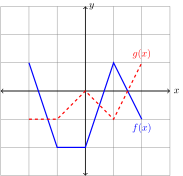
\includegraphics[width=0.6\columnwidth]{figures/0-3-fig3.pdf}
%                 \end{center}
%                 \caption{The functions $f(x)$ and $g(x)$ for Activity \ref{A:0.3.2}.}
%                 \label{f:A:0.3.2}
%             \end{figure}

            \begin{minipage}{0.5\columnwidth}
                \begin{center}
                    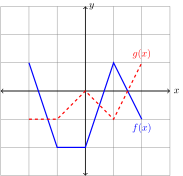
\includegraphics[width=0.9\columnwidth]{figures/0-3-fig3.pdf}
                \end{center}
            \end{minipage}
            \begin{minipage}{0.4\columnwidth}
                \begin{flalign*}
                    f(1) &= \underline{\hspace{1in}} \\
                    g(2) &= \underline{\hspace{1in}} \\
                    g(f(1)) &= \underline{\hspace{1in}} \\
                    f(g(1)) &= \underline{\hspace{1in}} \\
                    g(f(f(0))) &= \underline{\hspace{1in}}
                \end{flalign*}
                
            \end{minipage}
    \ea

\end{activity}
\begin{smallhint}
    \ba
        \item Start from the inside and work your way out.  The first two answers will be
            numbers and the next three will be functions.
        \item The numbers on the inside of the table are the $y$ values for the functions
            $f$ and $g$.  
        \item You're looking for the $y$ values that come out of these functions.
    \ea
\end{smallhint}
\begin{bighint}
    \ba
        \item On the function compositions, first evaluate the expression inside the
            parenthesis.  Then evaluate the outside.
        \item For an expression such as $f(g(-3))$, first evaluate $g(-3)$ and then
            substitute the answer into $f$.
        \item The same hints apply to the graphical version of the problem.
    \ea
\end{bighint}
\begin{activitySolution}
    \ba
        \item For $f(x) = x^2$ and $g(x) = x+8$
            \begin{flalign*}
                f(g(3)) &= f(11) = 121 \\
                g(f(3)) &= g(9) = 17 \\
                f(g(x)) &= f(x+8) = (x+8)^2 \\
                g(f(x)) &= g(x^2) = x^2 + 8 \\
                f(x)g(x) &=(x^2)(x+8) = x^3 + 8x^2 
            \end{flalign*}
        \item
            \begin{flalign*}
                f(-3) &= 3 \\
                g(3) &= 2 \\
                f(g(-3)) &= f(-2) = 1 \\
                f(g(f(-3))) &= f(g(3)) = f(2) = 1
            \end{flalign*}
        \item 
            \begin{flalign*}
                f(1) &= 1 \\
                g(2) &= 1 \\
                g(f(1)) &= g(1) = -1 \\
                f(g(1)) &= f(-1) = -2 \\
                g(f(f(0))) &= g(f(-2)) = g(1) = 1
            \end{flalign*}
    \ea
\end{activitySolution}


\aftera
